\chapter{烯烃的氧化与还原}\label{ch:b2:alkene-redox}

双组分环氧胶装于两管中：一管装着末端带有
环氧化物环的分子，即由两个碳原子和一个氧原子组成的三元环；另一管装胺。
两者混合后，张力较大的环相继打开，胶体凝固
成坚硬的网络。烯烃是制备此类环的原料，
也可用于制备羟基位置违背马氏规则的醇、具有指定几何构型的二醇，
以及那些曾帮助化学家判断双键在分子中位置的小片段。
本章在本科一年级分册亲电加成的基础上，
补充使双键被还原或被氧化的反应，
以及每一反应所带来的立体化学要求。

\begin{recall}
本科一年级分册内容：亲电加成、马氏规则、卤正离子、
顺式与反式加成、烯烃的水合、碳的氧化级别、
氢负离子供体、化学选择性、内消旋化合物与外消旋混合物、
立体专一反应。在\Cref{ch:b2:catalytic-cycles}中讨论了
威尔金森催化剂的氢化循环。
\end{recall}

\begin{omfigure}
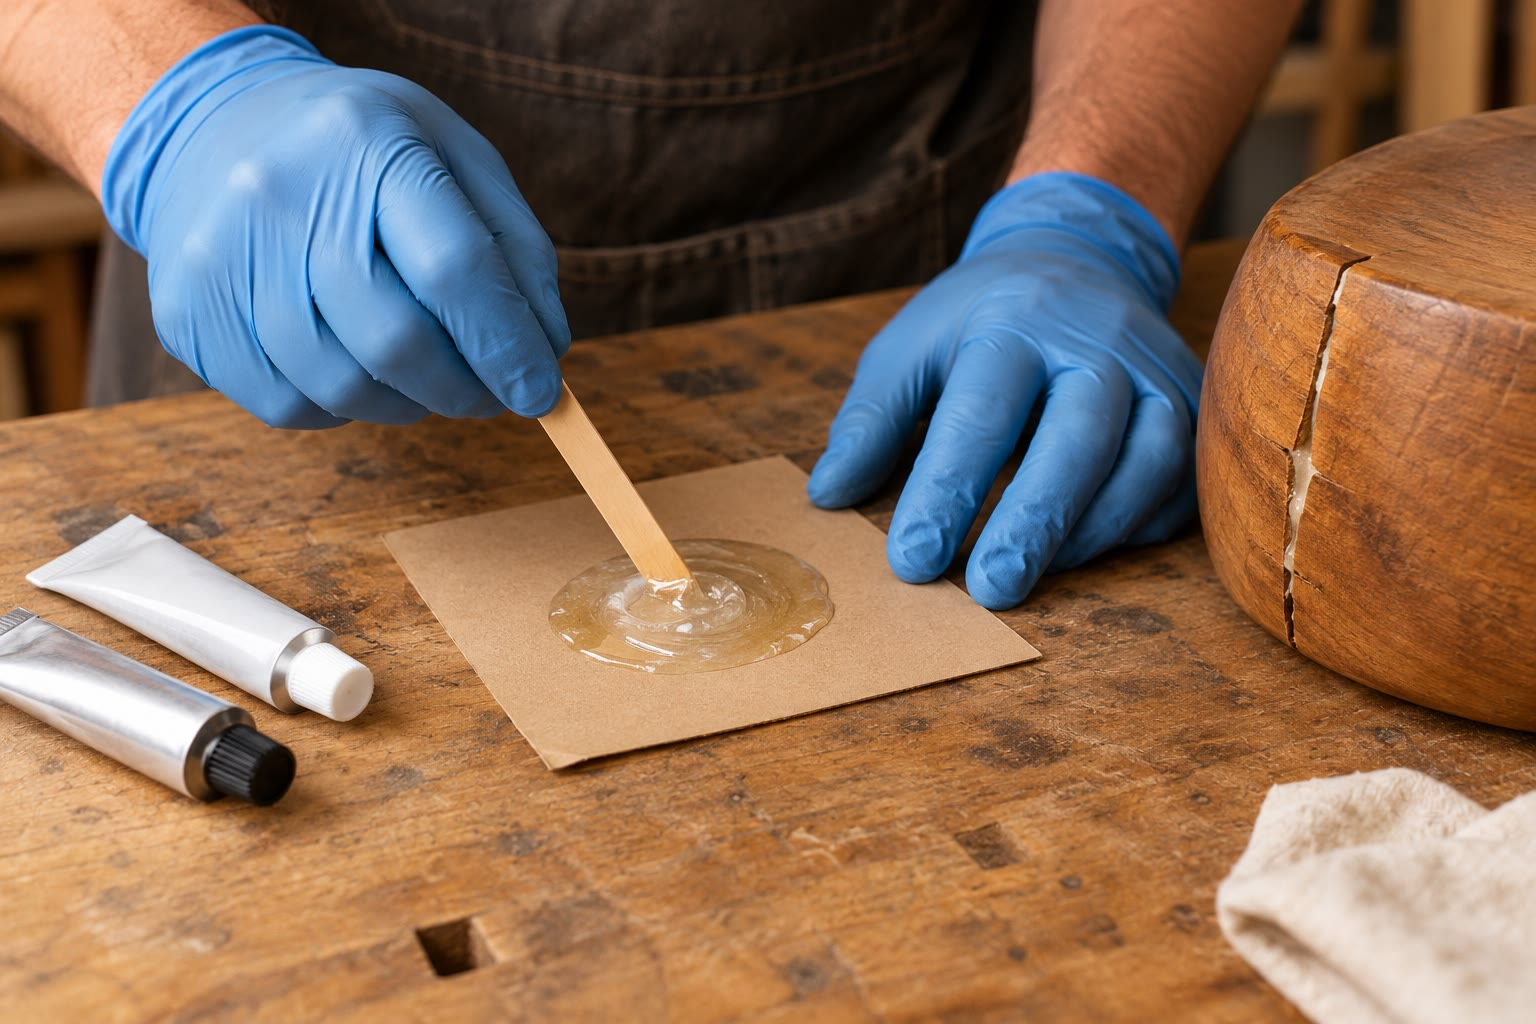
\includegraphics[width=0.6\linewidth]{images/book3/ai/b2-21-epoxy.jpg}

{\small 双组分环氧胶的混合：树脂（含环氧基）与
胺类固化剂一接触即发生反应，环被打开，分子连接成
固体网络。}
\end{omfigure}

\section{催化氢化}

\begin{definition}[催化氢化]\label{def:b2:alkene-redox:hydrogenation}
称\emph{催化氢化}\index{催化氢化}为在催化剂作用下，使氢气
加成到多重键上的反应。所用催化剂若为细分金属（钯碳、铂、镍），
则属多相催化；若为可溶配合物，如
威尔金森配合物，则属均相催化。
\end{definition}

在金属表面上，氢气与烯烃同时被吸附，\ce{H-H} 键断裂
生成表面氢原子，这些氢原子依次转移到烯烃的碳原子上，
而烯烃平躺在金属表面。

\begin{proposition}[顺式加成]\label{prop:b2:alkene-redox:syn-hydrogenation}
催化氢化使两个氢原子加到双键的同一侧。
炔烃在中毒的钯催化剂上氢化时，停在烯烃阶段，所得烯烃为
（\textit{Z}）异构体。
\end{proposition}

\begin{proof}[论证]
烯烃以一个面与催化剂结合，
两个氢原子都来自该面上的催化剂，这是顺式加成。炔烃时，加到
三键上的两个氢原子位于同侧、彼此为顺式，生成（\textit{Z}）-烯烃。部分
失活的催化剂（碳酸钙载钯，加入铅盐与喹啉）
与炔烃的结合远强于生成的烯烃，
因而烯烃在再次加成之前便离开表面。
\end{proof}

\section{硼氢化–氧化}

\begin{definition}[硼氢化]\label{def:b2:alkene-redox:hydroboration}
称\emph{硼氢化}\index{硼氢化}为使硼烷的 B--H 键加成到
\ce{C=C} 键上的反应；随后经碱性过氧化氢氧化，可将
烯烃转化为羟基位于取代较少碳原子上的醇，即
\emph{反马氏取向}\index{反马氏取向}。
\end{definition}

\begin{omfigure}
\setchemfig{atom sep=1.8em}
\schemestart[][west]
\chemfig{H_3C-[:30]CH=[:-30]CH_2}
\+ \chemfig{H-BH_2}
\arrow{->[顺式加成]}
\chemfig{H_3C-[:30]CH_2-[:-30]CH_2-[:30]BH_2}
\arrow{->[\ce{H2O2}][\ce{HO-}]}
\chemfig{H_3C-[:30]CH_2-[:-30]CH_2-[:30]OH}
\schemestop
\par\vspace{6pt}

{\small 丙烯的硼氢化–氧化。硼烷一步加成，硼加到
末端碳原子上，氢加到内侧碳原子上，两者位于同一面；氧化
以 \ce{OH} 取代硼，且构型保持。生成的是丙-1-醇，而非
酸催化水合所得的丙-2-醇。}
\end{omfigure}

\begin{proposition}[硼氢化的取向]\label{prop:b2:alkene-redox:hydroboration-regio}
硼加到双键中取代较少的碳原子上，氢加到取代较多的
碳原子上，该加成为顺式加成。
\end{proposition}

\begin{proof}[论证]
硼具有空的 p 轨道，是亲电试剂：在四中心过渡态中
（两个碳原子、硼与氢），硼的键略早于 C--H 键形成，另一个
碳原子上产生部分正电荷，取代较多的碳原子更能承载
这一正电荷；体积较大的硼基也偏向空间位阻较小的一端。两个新键
在同一面上协同形成，属顺式加成。
\end{proof}

\begin{proposition}[保持构型的氧化]\label{prop:b2:alkene-redox:retention}
烷基硼烷经碱性过氧化氢氧化，每个 C--B 键被
C--OH 键取代，碳原子上的构型保持不变。
\end{proposition}

\begin{proof}[论证]
氢过氧根离子加到硼上，随后烷基带着其电子对
从硼迁移到相邻的氧原子上，氢氧根随之离去；碳原子的
键在整个过程中始终位于同一侧。B--O 键水解，释放出醇。
\end{proof}

\section{环氧化物}

\begin{definition}[环氧化物]\label{def:b2:alkene-redox:epoxide}
称\emph{环氧化物}\index{环氧化物}（氧杂环丙烷）为含三元环的环醚，该环由
两个碳原子和一个氧原子构成。\emph{环氧化}\index{环氧化}是将烯烃转化为
环氧化物的反应，通常使用\emph{过氧酸}\index{过氧酸} \ce{RCO3H}，它将
一个氧原子转移到双键上。
\end{definition}

\begin{omfigure}
\setchemfig{atom sep=2em}
\schemestart
\chemfig{R-[:30]CH=[:-30]CH-[:30]R}
\+ \chemfig{Ar-C(=[2]O)-O-O-H}
\arrow{->}
\chemfig{[:-60]CH(-[:210]R)*3(-CH(-[:-30]R)-O-)}
\+ \chemfig{Ar-C(=[2]O)-OH}
\schemestop
\par\vspace{6pt}

{\small 过氧酸环氧化（Ar：例如 3-氯苯基）。过氧酸的末端
氧原子在一步反应中转移到双键上，两个 C--O 键
在同一侧生成。}
\end{omfigure}

\begin{proposition}[立体专一的环氧化]\label{prop:b2:alkene-redox:epoxidation}
过氧酸环氧化是立体专一的：(\textit{Z})-烯烃得到顺式环氧化物，
(\textit{E})-烯烃得到反式环氧化物。
\end{proposition}

\begin{proof}
氧原子通过一步协同过程转移到双键的一侧，在此过程中
双键不发生旋转，取代基的相对位置保持不变。
\end{proof}

\begin{proposition}[环氧化物的开环]\label{prop:b2:alkene-redox:opening}
亲核试剂从与氧原子相反的一侧进攻环氧化物的某一个碳原子，使其开环
（反式开环，该碳原子发生构型翻转）。在碱性条件下，亲核试剂进攻
位阻较小的碳原子；在酸性条件下，进攻取代程度较高的碳原子。
\end{proposition}

\begin{proof}[论证]
环张力使 C--O 键易于断裂。若亲核试剂较强且无酸存在，
开环为双分子取代反应，位阻最小的碳原子最易被进攻。
在酸中，氧原子被质子化；通向取代程度较高碳原子的 C--O 键
伸长最多，该碳原子带有较多的正电荷，即使是弱亲核试剂
（水、醇）也会在此处进攻，仍从背面进攻，因此仍为反式。
\end{proof}

\begin{omfigure}
\setchemfig{atom sep=2em}
\schemestart
\chemfig{[:-60]C(-[:210]H_3C)(-[:150]H_3C)*3(-CH_2-O-)}
\arrow{->[\ce{CH3O-}][\ce{CH3OH}]}[,1.4]
\chemfig{H_3C-C(-[2]CH_3)(-[6]OH)-CH_2-OCH_3}
\schemestop

\medskip
\schemestart
\chemfig{[:-60]C(-[:210]H_3C)(-[:150]H_3C)*3(-CH_2-O-)}
\arrow{->[\ce{CH3OH}][\ce{H+}]}[,1.4]
\chemfig{H_3C-C(-[2]CH_3)(-[6]OCH_3)-CH_2-OH}
\schemestop
\par\vspace{6pt}

{\small 甲醇使 2,2-二甲基环氧乙烷开环。上图为甲氧负离子条件：进攻
\ce{CH2}，位阻较小的碳原子。下图为酸性条件：进攻取代程度较高的碳原子，
该碳原子带有质子化环氧化物的大部分正电荷。}
\end{omfigure}

\section{双羟基化}

\begin{definition}[双羟基化]\label{def:b2:alkene-redox:dihydroxylation}
称\emph{双羟基化}\index{双羟基化}为将烯烃转化为 1,2-二醇的反应，
即在双键的每个碳原子上加入一个 \ce{OH} 基团。
\end{definition}

催化量的四氧化锇与再氧化剂共同使用，以及冷的稀高锰酸钾溶液，
均通过环状酯在同一侧加入两个氧原子，为顺式双羟基化。先环氧化
再在酸中与水开环，得到反式二醇。

\begin{proposition}[顺式与反式二醇]\label{prop:b2:alkene-redox:diols}
由 (\textit{Z})-2-丁烯出发，顺式双羟基化得到内消旋丁烷-2,3-二醇，环氧化路线
则得到外消旋的 (2\textit{R},3\textit{R}) 与 (2\textit{S},3\textit{S}) 二醇；由
(\textit{E})-2-丁烯出发，结果恰好互换。
\end{proposition}

\begin{proof}
在 (\textit{Z})-2-丁烯中，两个甲基位于同一侧。在一侧加入两个 \ce{OH}，
得到的二醇按原双键的重叠式构象书写时，
两个 \ce{OH} 位于一侧，两个甲基位于另一侧，一个镜面位于 C2 与 C3 之间，
即内消旋化合物。环氧化路线使两个 \ce{OH} 位于相反两侧（反式），
镜面消失；非手性环氧化物的两个碳原子被进攻的机会相等，
得到等量的两个对映异构体。对于 (\textit{E})-烯烃，
每一步都改变甲基之间的关系，因此结果互换。
\end{proof}

\begin{omfigure}
\begin{tikzpicture}[font=\small]
  \begin{scope}
    \draw[thick] (0,0) -- (0,1.2);
    \draw[thick] (0,1.2) -- (-0.7,1.45); \draw[thick] (0,1.2) -- (0.7,1.45);
    \node[anchor=east] at (-0.7,1.45) {\ce{HO}}; \node[anchor=west] at (0.7,1.45) {\ce{CH3}};
    \draw[thick] (0,0) -- (-0.7,0.25); \draw[thick] (0,0) -- (0.7,0.25);
    \node[anchor=east] at (-0.7,0.25) {\ce{HO}}; \node[anchor=west] at (0.7,0.25) {\ce{CH3}};
    \node[anchor=south] at (0,1.25) {\scriptsize H};
    \node[anchor=north] at (0,-0.05) {\scriptsize H};
    \draw[densely dashed, omThm] (-1.6,0.6) -- (1.6,0.6);
    \node at (0,-1.0) {顺式：内消旋};
  \end{scope}
  \begin{scope}[xshift=6.5cm]
    \draw[thick] (0,0) -- (0,1.2);
    \draw[thick] (0,1.2) -- (-0.7,1.45); \draw[thick] (0,1.2) -- (0.7,1.45);
    \node[anchor=east] at (-0.7,1.45) {\ce{HO}}; \node[anchor=west] at (0.7,1.45) {\ce{CH3}};
    \draw[thick] (0,0) -- (-0.7,0.25); \draw[thick] (0,0) -- (0.7,0.25);
    \node[anchor=east] at (-0.7,0.25) {\ce{H3C}}; \node[anchor=west] at (0.7,0.25) {\ce{OH}};
    \node[anchor=south] at (0,1.25) {\scriptsize H};
    \node[anchor=north] at (0,-0.05) {\scriptsize H};
    \node[align=center] at (0,-1.1) {反式：一种对映异构体 \\（与其镜像一同生成）};
  \end{scope}
\end{tikzpicture}

{\small 由（\textit{Z}）-丁-2-烯生成的两种丁-2,3-二醇，示意图（竖直的 C2--C3
键，每个碳两侧的基团分列左右）。顺式加成使两个
\ce{OH} 位于同侧：存在内部对称面（虚线），为内消旋化合物。反式加成使两者
位于异侧，得到手性二醇，与其对映体一同生成。}
\end{omfigure}

\section{氧化裂解}

\begin{definition}[氧化裂解]\label{def:b2:alkene-redox:cleavage}
称\emph{氧化裂解}\index{氧化裂解}为断开 \ce{C=C} 双键
的两根键、并使每个碳转化为羰基或羧基的反应。在
\emph{臭氧解}\index{臭氧解}中，烯烃与臭氧反应，中间体
臭氧化物在第二步，即后处理中被分解。
\end{definition}

\begin{proposition}[臭氧解的产物]\label{prop:b2:alkene-redox:ozonolysis}
臭氧解将每个 \ce{C=C} 键断裂为两个 \ce{C=O} 基团。采用还原性后处理
（锌和酸，或二甲硫醚）时，连有一个氢的碳生成醛；采用氧化性后处理
（过氧化氢）时，生成羧酸。连有两个碳基团的碳
在两种情况下均生成酮。
\end{proposition}

\begin{proof}[证明]
臭氧加成到双键上，中间体重排，C--C 键断裂，生成
臭氧化物，其中每个原烯烃碳与两个氧原子相连。后处理将其还原为
两个羰基化合物，或将醛进一步氧化。中间步骤
在本阶段不加证明地承认。
\end{proof}

\begin{omfigure}
\setchemfig{atom sep=2em}
\schemestart
\chemfig{H_3C-[:30]C(-[:90]CH_3)=[:-30]CH-[:30]CH_3}
\arrow{->[1. \ce{O3}][2. \ce{Zn}, \ce{H+}]}[,1.8]
\chemfig{H_3C-C(=[2]O)-CH_3}
\+
\chemfig{H-C(=[2]O)-CH_3}
\schemestop
\par\vspace{6pt}

{\small 2-甲基丁-2-烯在还原性后处理下的臭氧解生成丙酮和
乙醛。将两个羰基碳以双键相连，可
重建该烯烃。}
\end{omfigure}

\begin{method}[确定双键的位置]\label{met:b2:alkene-redox:locate-double-bond}
\begin{enumerate}
  \item 列出臭氧解所得羰基片段，并数出其碳原子数，二者之和
        应等于烯烃的碳原子数。
  \item 每个 \ce{C=O} 中的碳原本是双键碳：将两个 \ce{C=O} 替换为
        一个 \ce{C=C}，即可连接各片段。
  \item 若为环状结构，则得到一个含两个羰基的分子；连接其两端即可。
  \item 用分子式和不饱和度进行校验。
\end{enumerate}
\end{method}

热的浓高锰酸盐同样可裂解双键，生成酸和酮；高碘酸钠
可将 1,2-二醇裂解为两个羰基化合物，这是经二醇的一条较温和途径。

\begin{method}[选择烯烃的试剂]\label{met:b2:alkene-redox:choose-reagent}
\begin{center}
\small
\renewcommand{\arraystretch}{1.15}
\begin{tabular}{lll}
目标产物 & 试剂 & 立体化学、取向 \\ \hline
烷烃 & \ce{H2}, Pd/C & 顺式 \\
马氏醇 & \ce{H2O}, 酸 & 经由碳正离子 \\
反马氏醇 & \ce{BH3}, 再 \ce{H2O2}, \ce{HO-} & 顺式 \\
环氧化物 & 过氧酸 & 立体专一 \\
顺式二醇 & \ce{OsO4}（催化量）或冷的 \ce{MnO4-} & 顺式 \\
反式二醇 & 过氧酸，再 \ce{H2O}, 酸 & 反式 \\
两个羰基 & \ce{O3}，再 \ce{Zn}/酸 & 裂解 \\
\end{tabular}
\end{center}
\end{method}

\begin{safety}{\ghs[5mm]{GHS02}\,\ghs[5mm]{GHS03}\,\ghs[5mm]{GHS05}\,\ghs[5mm]{GHS06}}
四氧化锇易挥发，毒性很强（会损伤眼睛），须以催化量
溶于溶液中，并在通风橱中使用。过氧酸和过氧化氢是氧化剂，
加热或浓缩时可能剧烈分解；硼烷溶液易燃；
臭氧有毒，须在通风橱中产生和使用。
% ledger: ghs:OsO4, ghs:mCPBA, ghs:BH3-THF, ghs:O3, ghs:NaIO4
\end{safety}

\section{练习}

\begin{exercise}[$\star$]\label{exo:b2:alkene-redox:1}
求 1-甲基环己烯分别与下列试剂反应的产物：\ce{H2}/Pd；\ce{H2O}/\ce{H+}；
\ce{BH3} 再 \ce{H2O2}/\ce{HO-}；过氧酸；\ce{OsO4}（催化量）；\ce{O3} 再
\ce{Zn}/\ce{H+}。
\end{exercise}

\begin{exercise}[$\star$]\label{exo:b2:alkene-redox:2}
由 2-甲基丙烯经硼氢化–氧化得到哪种醇？酸催化
水合又得到什么？
\end{exercise}

\begin{exercise}[$\star$]\label{exo:b2:alkene-redox:3}
画出由（\textit{E}）-丁-2-烯生成的环氧化物。它是否具有手性？
\end{exercise}

\begin{exercise}[$\star$]\label{exo:b2:alkene-redox:4}
求己-3-烯臭氧解的产物，分别采用还原性后处理和
氧化性后处理。
\end{exercise}

\begin{exercise}[$\star\star$]\label{exo:b2:alkene-redox:5}
求由（\textit{Z}）-丁-2-烯生成的二醇：（a）与 \ce{OsO4} 反应；（b）与过氧酸
反应后再经水溶液酸处理。哪一个因为是内消旋化合物而无旋光性，
哪一个因为是外消旋混合物而无旋光性？
\end{exercise}

\begin{exercise}[$\star\star$]\label{exo:b2:alkene-redox:6}
2,2-二甲基环氧乙烷在酸催化下与水开环，也可在氢氧根作用下开环。两条
路线得到的产物是否相同？请说明理由。
\end{exercise}

\begin{exercise}[$\star\star$]\label{exo:b2:alkene-redox:7}
如何由己-3-炔制备（\textit{Z}）-己-3-烯？
\end{exercise}

\begin{exercise}[$\star\star$]\label{exo:b2:alkene-redox:8}
烯烃 \ce{C7H14} 经还原性后处理的臭氧解，得到丙酮和丁醛。
求其结构。
\end{exercise}

\begin{exercise}[$\star\star$]\label{exo:b2:alkene-redox:9}
提出由己-1-烯合成己-1-醇的路线，并说明酸催化
水合为何会失败。
\end{exercise}

\begin{exercise}[$\star\star\star$]\label{exo:b2:alkene-redox:10}
柠檬烯含有一个三取代的环双键和一个二取代的环外双键
（\ce{C(CH3)=CH2}）。哪一个先与一当量过氧酸反应，哪一个与
一当量体积庞大的硼烷反应？请说明理由。
\end{exercise}

\begin{exercise}[$\star\star\star$]\label{exo:b2:alkene-redox:11}
由环己烯制备反式环己烷-1,2-二醇，并制备顺式环己烷-1,2-二醇。
\end{exercise}

\begin{exercise}[$\star\star\star$]\label{exo:b2:alkene-redox:12}
某化合物 \ce{C6H10} 可吸收一当量 \ce{H2}，其经还原性后处理的臭氧解
仅得到一种产物，即己二醛 \ce{OHC-(CH2)4-CHO}。试确定其结构。
\end{exercise}

\section{问题：鉴定一种萜烯}

\begin{problem}[{周末问题——柠檬烯的化学式与不饱和度，及其
氢化、臭氧解的片段，以及其两个
双键的选择性反应}]
\label{pb:b2:alkene-redox:1}
柠檬烯带有橙皮的香气，化学式为 \ce{C10H16}。其
结构为 1-甲基-4-（丙-1-烯-2-基）环己-1-烯：环上双键带有甲基，
环上相对的碳原子连有环外的 \ce{C(CH3)=CH2} 基团。$R =
\qty{8.314}{J/(K.mol)}$；摩尔质量（\unit{g/mol}）：C 12.011，H 1.008。
% ledger: aw:C, aw:H, const:R, ghs:limonene

\medskip
\noindent\textbf{第一部分——化学式与氢化。}
\begin{enumerate}
  \item 求柠檬烯的摩尔质量。
  \item 求其不饱和度。
  \item 它含有几个环、几个双键？
  \item 写出其在钯催化下的氢化反应式（包括产物）。
  \item 求 \qty{1.00}{g} 柠檬烯所吸收的氢气的物质的量。
  \item 求该氢气在 \qty{25}{\degreeCelsius} 和 \qty{1.00}{bar} 下的体积。
  \item 产物是否具有手性？
\end{enumerate}

\medskip
\noindent\textbf{第二部分——臭氧解。}
\begin{enumerate}[resume]
  \item 经还原性后处理的臭氧解得到哪些片段？（数一数碳原子。）
  \item 为何环双键只生成一个分子，而不是两个？
  \item 哪一个片段以气体或挥发性液体的形式逸出？
  \item 若采用氧化性后处理，产物会有何不同？
  \item 说明如何由这些片段确定两个双键的位置。
  \item 柠檬烯有几个手性碳原子？臭氧解是否保留其手性？
\end{enumerate}

\medskip
\noindent\textbf{第三部分——硼氢化。}
\begin{enumerate}[resume]
  \item 与一当量体积庞大的硼烷反应时，哪一个双键发生反应？为何如此？
  \item 画出氧化后的产物。
  \item 所得醇是伯醇、仲醇还是叔醇？
  \item 为何将该取向称为反马氏取向？
  \item 在新生成的手性碳原子上，可形成几种立体异构体？
  \item 若要使 \ce{OH} 落在同一双键上取代程度较高的碳原子上，
        应选用哪一种试剂？
\end{enumerate}

\medskip
\noindent\textbf{第四部分——环氧化。}
\begin{enumerate}[resume]
  \item 与一当量过氧酸反应时，哪一个双键发生反应？为何如此？
  \item 画出环氧化物。
  \item 在酸性条件下用水开环：水进攻哪一个碳原子？
  \item 画出该二醇，并给出其两个 \ce{OH} 的相对取向。
  \item 如何得到该二醇的另一种非对映异构体？
  \item 求 \qty{1.00}{g} 柠檬烯所吸收的氢气在
        \qty{25}{\degreeCelsius} 和 \qty{1}{bar} 下的体积。
\end{enumerate}
\end{problem}
